%%%%%%%%%%%%%%%%%%%%%%preface.tex%%%%%%%%%%%%%%%%%%%%%%%%%%%%%%%%%%%%%%%%%
% sample preface
%
% Use this file as a template for your own input.
%
%%%%%%%%%%%%%%%%%%%%%%%% Springer %%%%%%%%%%%%%%%%%%%%%%%%%%

\preface

%% Please write your preface here
% Use the template \emph{preface.tex} together with the Springer document class SVMono (monograph-type books) or SVMult (edited books) to style your preface in the Springer layout.

% A preface\index{preface} is a book's preliminary statement, usually written by the \textit{author or editor} of a work, which states its origin, scope, purpose, plan, and intended audience, and which sometimes includes afterthoughts and acknowledgments of assistance. 

% When written by a person other than the author, it is called a foreword. The preface or foreword is distinct from the introduction, which deals with the subject of the work.

% Customarily \textit{acknowledgments} are included as last part of the preface.

%\paragraph{Origin}

The reader will find in this monograph a series of tutorials and advanced topics originally written over the last ten years as documentation parts for the \Digraph collection of Python modules. These programming resources -- like the \texttt{outrankingDigraphs} module -- were essentially used for the preparation and illustration of the Algorithmic Decision Theory course taught at the University of Luxembourg from 2010 to 2020. Some resources, like the \texttt{randomNumbers} module, served for preparing and illustrating the Lectures of a Computational Statistics Course. Curious readers will iscover some resources --the \texttt{arithmetics} module-- used for preparing and illustrating a first Semester Course on Discrete Mathematics.

%\paragraph{Scope}

The \Digraph Python programming resources are useful in the field of Algorithmic Decision Theory and more specifically for the outranking approach of Multiple Criteria Decision Aid (MCDA). In this latter scientific filed, we address essentially three kinds of usage.
\begin{enumerate}[topsep=3pt,partopsep=0pt]
\item First, we present methods an illustrate computing tools for solving either a multiple criteria best choice selection or a dual worst choice rejection problem, mainly interesting for management or social choice studies.
\item We also address the problem of how to list a set of items with multiple incommensurable performance criteria either from the best to the worst (ranking problem) or from the worst to the best (ordering problem), mainly interesting for schedulers or designers of recommender systems.
\item The third kind of usage should mainly be of interest for performance auditors, as we present methods and tools for relative or absolute quantiles rating of multiple criteria performance records. 
\end{enumerate}

It is necessary to mention that the \Digraph ressources do not provide a professional Python software library. The collection of Python modules, we describe in this book, was not built following any professional software development methodology. The design of classes and methods was kept as simple and elementary as was opportune for the author. Sophisticated and cryptic overloading of classes, methods and variables is more or less avoided all over. A simple copy, paste and ad hoc customisation development strategy was generally preferred. As a consequence, the \Digraph modules keep a large part of independence and are hence easier to maintain and adapt.  Furthermore, the development of the \Digraph modules being spread over two decades, our programming style did evolve with our growing experience and the changes and enhancement coming up with the ongoing new releases of the standard Python3 libraries. The required backward compatibility necessarily introduced so with time some notation and programming technique changes.

%\paragraph{Purpose}

The purpose of this book is to present in a single monograph the many scientific enhancements the author has contributed over the past two decades to the outranking approach-based multiple criteria decision aid field - and that are either left unpublished or published in very specialised media only and difficult to access.  

%\paragraph{Plan}

This monograph should provide the reader with a self-contained series of tutorials which explain how to solve multiple criteria selection, as well as ranking or rating decision problems. If successful in this aim, the curious reader will effectively install the \Digraph programming resources on their laptop and try out and redo for themselves the proposed computations.

%\paragraph{Intended audience}

The material in this book is valuable for master students and doctoral candidates in Computer Science, Mathematics, Engineering Sciences or Computational Management Sciences taking a course on Algorithmic Decision Theory, Multiple Criteria Decision Aid or Decision Analysis. Some experience in computer programming, in particular with Python, will assist the reader, but it is not a prerequisite. The many coding examples shown throughout the text are purposely kept elementary from a programming point of view. 

Chapters presenting methods and tools for ranking multiple criteria performance records from best to worst --especially when facing big performance tableaux-- may be of interest to designers of web recommender systems. 

Similarly, the relative and absolute quantiles-rating methods and tools discussed and illustrated will be of practical interest for private or public performance auditors.

Finally, the monograph does not provide any mathematical developments or proofs. Those readers interested in the mathematical background of our decision methods and tools are invited to consult the references provided at chapter level. Full texts of most of these references may be downloaded from the \href{https://orbilu.uni.lu/}{https://orbilu.uni.lu/} repository of the University of Luxembourg. 

\paragraph{Acknowledgments}

This monograph contains many ideas, methods and tools that are not only the author’s. They have been shared and enhanced with friends, colleagues and students: 

\vspace{0.5cm}
\begin{minipage}{7cm}
\emph{Denis Bouyssou, Luis Dias,}\\ 
\emph{Claude Lamboray, Patrick Meyer,}\\
\emph{Vincent Mousseau, Alex Olteanu,}\\
\emph{Marc Pirlot, the late Bernard Roy,}\\
\emph{Alexis Tsouki\`as, Thomas Veneziano,}\\
and especially,\\
\emph{the late Marc Roubens}.
\end{minipage}\quad
\begin{minipage}{3cm}
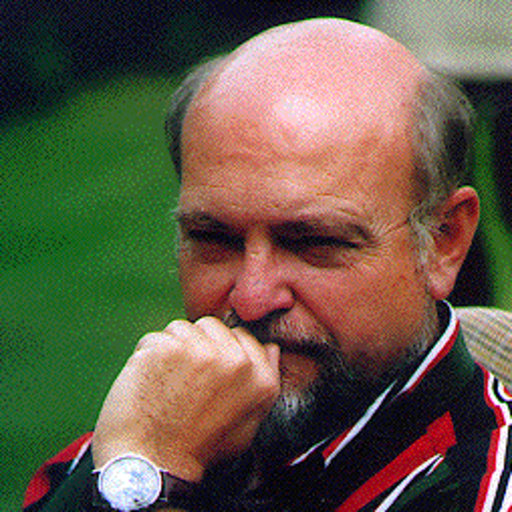
\includegraphics[width=3cm]{Figures/Marc-Roubens.jpg} \\
{\small \emph{Marc Roubens}}
\end{minipage}

\vspace{0.3cm}
Their help is gratefully acknowledged.

\vspace{\baselineskip}
\begin{flushright}\noindent
Luxembourg, 2021\hfill {\it Raymond Bisdorff}\\
%month year\hfill {\it Firstname  Surname}\\
\end{flushright}


